\chapter{Electromagnetic Methods}\label{ch:EMmethods}

\section{Key Concepts}
\begin{itemize}
    \item Maxwell's equations (at least in a general way, e.g., Gauss's law of electricity states that the electric field on an enclosed surface is related to the charges contained within the volume enclosed by that surface and Faraday's law suggests that a time varying magnetic field causes a spatial change in the electric field.) Note all del (upside down triangle) denotes is a spatial variation in a parameter one way or another.

    \item What are the wave equation, diffusion equation, and Helmholtz
    equations. What assumptions help define them (e.g., for magnetic induction we assume the conductivity is ? than the electric permittivity).

    \item What is the difference between a time domain and frequency domain
    method?

    \item What is magnetic induction (you should be able to express this in
    words as well as a simple equation)?

    \item What are the implications of the circuit analogy (i.e., what are the
    currents in the conductor and receiver sensitive to and how do they relate
    to the resistivity of the Earth)?

    \item What are skin depth, characteristic impedance, apparent resistivity,
    surface impedance (and how are they calculated\ldots)?

    \item What are the 1-D generalizations for MT?

    \item What are electrical conductivities of typical earth materials?  How do
    we estimate effective conductivity for mixed phases?
\end{itemize}

\section{Mathematical symbols and units}
\begin{table}[hbt]
    \centering
    \begin{threeparttable}
    \caption{Definitions of symbols.\vspace{2pt}}
    \label{tab:emsym}
    \begin{tabular}{@{}cll@{}}
        \toprule
        Symbol &
        Quantity &
        SI Unit \\
        \midrule
        $t$             & time                          & second, \si{s} \\
        $x$, $y$, $z$   & distance                      & meter, \si{m} \\
        $\tau$          & period                        & s \\
        $f$             & frequency                     & hertz, \si{s^{-1}} \\
        $\omega$        & angular frequency ($\omega = 2 \pi f$) & \si{rad.s^{-1}} \\
        $\lambda$       & wavelength                    & \si{m} \\
        $k$             & wavenumber ($k = 2\pi \lambda^{-1}$)
            & radians m$^{-1}$ \\

        $q$ ($Q$)       & single (total) electric charge    & coulomb, \si{C} \\
        $\rho_{f}$      & electric charge density       & \si{C.m^{-2}} \\
        $U$, $V$        & electric potential, voltage   & volt, \si{V} \\
        $\mathcal{E}$      & electromotive force           & V \\
        $I$             & electric current              & ampere, $\si{A} = \si{C.s^{-1}}$ \\
        $R$             & resistance                    & ohm, \si{\Omega} \\
        $L$             & inductance                    & henry, \si{H} \\
        $C$             & capacitance                   & farad, \si{F} \\
        $Z$             & complex impedance             & \si{\Omega} \\

        $\vb{D}$       & electric displacement/flux density    & \si{C.m^{-2}} \\
        $\vb{E}$       & electric field strength       & \si{V.m^{-1}} \\
        $\vb{B}$       & magnetic induction/flux density   & tesla,
            \si{T} = \si{Wb.m^{-2}} = \si{V.s.m^{-2}} \\
        $\vb{H}$       & magnetic field strength       & \si{A.m^{-1}} \\
        $\Phi_{B}$      & magnetic flux                 & weber, $\si{Wb} = \si{V.s}$ \\
        $\vb{J}$       & electric current density      & \si{A.m^{-2}} \\

        $\rho$          & electrical resistivity        & \si{\Omega.m} \\
        $\sigma$        & electric conductivity         & \si{S.m^{-1}}; 
        siemens, $\si{S} = \si{\Omega^{-1}}$ \\
        $\epsilon$      & electrical permittivity, dielectric constant &
        \si{F.m^{-1}} \\
        $\mu$           & magnetic permeability         & \si{H.m^{-1}} \\
        \bottomrule
    \end{tabular}
    \begin{tablenotes}
        \item Notes: Scalar quantities are written as $B$, while vectors are written as $\vb{B}$.
        \item The unit of conductance, \si{S}\ or \si{\Omega^{-1}}, is also called a mho (for ohm backward) and can be denoted by
        \si{\mho}.
    \end{tablenotes}
    \end{threeparttable}
\end{table}

OK, I'm going to stop right here and rant for a minute.  I HATE the units in
electromagnetics.  Almost every physical quantity is given its own unit.  But
almost none of them are fundamental, by which I mean a metric (distance and
time) or a measurable quantity that is directly derived from the nature of a
particle.  The one exception is the unit for charge, the Coulomb, which is the
electrostatics analog to the mass of a particle.  What I am calling a
fundamental unit here is sometimes referred to as a base unit.

The quantities in the above table are the ones commonly used because it is
useful to know what units are standard\ldots but what the {\it hell} is a henry?
How about a volt per ampere?  And how does a tesla relate to a weber?

The following below is a guide that will help relate some of these properties to
each other and hopefully help you gain some insight into the physical meaning of
these quantities.  It will also be helpful as you check units of solutions to
derivations.
\begin{table}[hbt]
  \footnotesize
  \caption{Units guide.}
  \label{tab:symguide}
  \begin{tabularx}{\textwidth}{@{}cllX@{}}
    \toprule
    Unit &
    Name &
    Other definitions &
    Comments \\
    \midrule
    \multicolumn{4}{c}{\it base units} \\
    \si{m}   & meter      & {}    & distance (metric) \\
    \si{s}   & second     & {}    & time (metric) \\
    \si{kg}  & kilogram   & {}    & mass (fundamental quantity) \\
    \si{C}   & coulomb    & {}    & charge (fundamental quantity) \\
    \multicolumn{4}{c}{\it derived units} \\
    \si{N}   & newton     & $\si{N} = \si{kg.m.s^{-2}}$                     & force \\
    \si{J}   & joule      & $\si{J} = \si{N.m} = \si{kg.m^{2}.s^{-2}}$      & energy \\
    \si{W}   & watt       & $\si{W} = \si{J.s^{-1}} = \si{kg.m^{2}.s^{-3}}$ & power \\
    \si{A}   & ampere     & $\si{A} = \si{C.s^{-1}}$                        & current (think of it like a charge velocity) \\
    \si{V}   & volt       & $\si{V} = \si{W.A^{-1}} = \si{J.C^{-1}} =
        \si{kg.m^{2}.s^{-2}.C^{-1}}$ &
        potential (it is the energy contained per charge) \\
    \si{\Omega} & ohm     & $\si{\Omega} = \si{V.A^{-1}} = \si{W.A^{-2}} = \si{N.C^{-1}} =
        \si{kg.m^{2}.s^{-2}.C^{-2}}$ &
        resistance (the difficulty in moving a charge, force per unit charge) \\
    \si{S}, \si{\mho} & siemens, \si{mho} & $\si{S} = \si{\Omega^{-1}} = \si{A.V^{-1}} = \si{A.W^{-1}} = \si{C.N^{-1}} = \si{s^{2}.C^{2}.kg^{-1}.m^{-2}}$ &
        conductance (if resistance is the difficulty in moving a charge, the
        conductance is the ease) \\
    \si{H}       & henry         & $\si{H} = \si{\Omega.s} = \si{V.s.A^{-1}} =
        \si{J.A^{-2}} = \si{kg.m^{2}.C^{-2}}$ & 
        inductance (decreasing resistance with time)\\
    \si{F}       & farad         & $\si{F} = \si{s.\Omega^{-1}} = \si{A.s.V^{-1}} = 
        \si{J.V^{-2}} = \si{s^{2}.C^{2}.kg^{-1}.m^{-2}}$ &
        capacitance (increasing resistance with time) \\
    \si{T}       & tesla         & $\si{T} = \si{V.s.m^{-2}} = \si{kg.A^{-1}.s^{-1}} =
        \si{N.A^{-1}.m^{-1}} = \si{kg.C^{-1}.s^{-1}}$ &
        magnetic induction \\
    \si{Wb}      & weber         & $\si{Wb} = \si{T.m^{-2}} = \si{V.s} = \si{J.A^{-1}} =
        \si{W.C^{-1}} = \si{kg.m^{2}.s^{-3}.C^{-1}}$ &
        magnetic flux (the power per unit charge) \\
    \bottomrule
  \end{tabularx}
\end{table}


\section{Maxwell's equations}
One of the greatest contributions to modern physics was the recognition that all
the observations governing electrical and magnetic systems could be linked
through four general laws (Maxwell's Equations).  Many of these were originally
developed as separate laws, but in a less general form.  Maxwell's insight
helped spur the development of both quantum mechanics and relativity.  So
without further ado, Maxwell's Equations (for macroscopic systems):
\begin{align}
    \div \vb{D} & = \rho_{f}; & \text{Gauss's law of electricity} \\
    \div \vb{B} & =  0; & \text{Gauss's law of magnetism} \\
    \curl \vb{E} & = -\pdv{\vb{B}}{t};
        & \text{Faraday's law} \\
    \curl \vb{H} & = \vb{J} + \pdv{\vb{D}}{t}.
        & \text{Ampere's law}
\end{align}
The above expressions are in differential form, but we can also write them in
integral form, which is convenient for some derivations:
\begin{align}
    \cint{S} \vb{D} \cdot \dd{\vb{A}} & = Q(V); &
        \text{Gauss's law of electricity} \\
    \cint{S} \vb{B} \cdot \dd{\vb{A}} & = 0; &
        \text{Gauss's law of magnetism} \\
    \cint{C} \vb{E} \cdot \dd{\vb{\ell}} & = - \dv{}{t} \fint{S}{}
        \vb{B} \cdot \dd{\vb{A}}; &
        \text{Faraday's law} \\
    \cint{C} \vb{H} \cdot \dd{\vb{\ell}} & = I_{f} + \fint{S}{}
        \pdv{\vb{D}}{t} \cdot \dd{\vb{A}}. &
        \text{Ampere's law}
\end{align}
The the free and bound charges within the volume $V$ is given by $Q$.

For isotropic materials with uniform electrical polarization and magnetization
we can write the following general relations;
\begin{align}
    \vb{D} & = \epsilon \vb{E}; \\
    \vb{B} & = \mu \vb{H}; \mbox{ and} \\
    \vb{J} & = \sigma \vb{E}.
\end{align}

It is also handy to know the Lorentz force,
\begin{equation}
    \vb{F} = q[\vb{E} + \vb{v} \times \vb{B}],
\end{equation}
which is the force on a charge as it moves through an electric and magnetic
field.

There is a lot of vector calculus in electromagnetics.  If you are unfamiliar
or need a refresher, I've included a few notes in an appendix.

\begin{framed}
    {\bf Aside:} In many ways $D$ and $H$ are artificial fields related to macroscopic
    approximations of microscopic processes occurring within materials.  In free
    space the electric permittivity, $\epsilon_0$, and magnetic permeability,
    $\mu_0$ are related to the speed of light, $c$ by
    \begin{equation*}
        c^2 = (\epsilon_0 \mu_0)^{-1}.
    \end{equation*}
    In the SI system, $\mu_0 = 4 \pi \times 10^{-7}$.
\end{framed}


\subsection{Wave equation}
There are two general partial differential equations (PDE's) that use for the
electromagnetic (EM) techniques discussed in these notes.  The first is the
wave equation and describes wave propagation in space and time.  We will start
by deriving the wave equation as it pertains to EM. 

We start by assuming our medium is isotropic with uniform properties.  This will
allow us to remove $D$'s and $B$'s from our Maxwell's equations; hence, we can
write Faraday's and Ampere's Laws as
\begin{align}
    \curl \vb{E} & = -\mu \pdv{\vb{H}}{t}, \\
    \curl \vb{H} & = \sigma \vb{E} + \epsilon \pdv{\vb{E}}{t}.
\end{align}
Taking the curl of Faraday's Law,
\begin{align*}
    \curl \curl \vb{E} & = \curl \left( -\mu \pdv{\vb{H}}{t} \right) \\
        & = -\mu \pdv{}{t} \left( \curl \vb{H} \right).
\end{align*}
We can greatly simplify our life by removing $H$ using Ampere's Law,
\begin{equation*}
    \curl \curl \vb{E} 
        = - \mu \pdv{}{t} \left( \sigma \vb{E} + \epsilon \pdv{\vb{E}}{t} \right).
\end{equation*}
Applying the vector identity $\curl \curl \vb{A} = \grad (\div \vb{A}) -
\nabla^2 \vb{A}$ and assuming that we are in a region with no free charges
(i.e.\ $\div E = 0$), we arrive at a form of the {\it wave equation},
\begin{equation}
    \nabla^{2} \vb{E} = \mu \sigma \pdv{\vb{E}}{t} + \mu \epsilon \pdv[2]{\vb{E}}{t}.
    \label{eq-Ewave}
\end{equation}

We can use a similar procedure to derive the wave equation for $H$,
\begin{equation}
    \nabla^{2} \vb{H} = \mu \sigma \pdv{\vb{H}}{t} + \mu \epsilon \pdv[2]{\vb{H}}{t}.
    \label{eq-Hwave}
\end{equation}

\begin{framed}
    {\bf Aside:} To derive the wave equation above, we assumed a uniform and
    isotropic medium.  In a uniform and isotropic medium the properties of the
    medium are constants.  Mathematically this is expressed as $\grad \sigma =
    0$.  Had this not been the case, $\sigma$ is a tensor and $\div (\sigma
    \vb{E})$ is no longer zero,
    \begin{equation*}
        \div (\sigma \vb{E}) = \sigma \div \vb{E} + \vb{E} \div{\sigma} =
        \vb{E} \div \sigma.
    \end{equation*}
    Thus the PDE is more complex.  If $\sigma$ is isotropic, but not
    homogeneous, we can still use the above formulation for the wave equation
    within layers with thicknesses small enough that the changes in $\sigma$ may
    be ignored.
\end{framed}


\subsection{Diffusion equation}
Diffusion is an important process arising in many physical situations.  Two
examples include the divergence of heat or chemical concentration away from a
source.  EM waves can also be governed by the diffusion equation when
displacement currents can be ignored (i.e.\ $\dd{D}/\dd{t} = 0$).  If we apply this
condition to Equations~\ref{eq-Ewave} and \ref{eq-Hwave}, we arrive at the
diffusion equation
\begin{align}
    \nabla^2 \vb{E} & = \mu \sigma \pdv{\vb{E}}{t} \\
    \nabla^2 \vb{H} & = \mu \sigma \pdv{\vb{H}}{t}.
    \label{eq-diffusion}
\end{align}
In order to ignore displacement currents, $\sigma \gg \omega \epsilon$.  This
approximation is called the {\it quasi-static approximation}.  We explore the
implications of the quasi-static approximation a bit more thoroughly in the
section on frequency domain techniques.


\section{Electromagnetic techniques}
All electromagnetic techniques from geophysics utilize Maxwell's Equations
albeit with differing assumptions to exploit the behaviors of materials when
exposed to varying frequencies of electromagnetic radiation.  On one extreme is
{\it ground penetrating radar} (GPR) which uses high frequency EM radiation in
10~MHz to 1~GHz (10$^7$ to 10$^9$~Hz).  On the other extreme is geomagnetic
depth sounding which may use extremely long periods of EM radiation extending to
years ($>10^{-6}$~Hz).  Yes, you read that right, frequencies spanning 15+
orders of magnitude (Figure~\ref{fig:spectrum}).
\begin{figure}[hp]
  \centerline{
    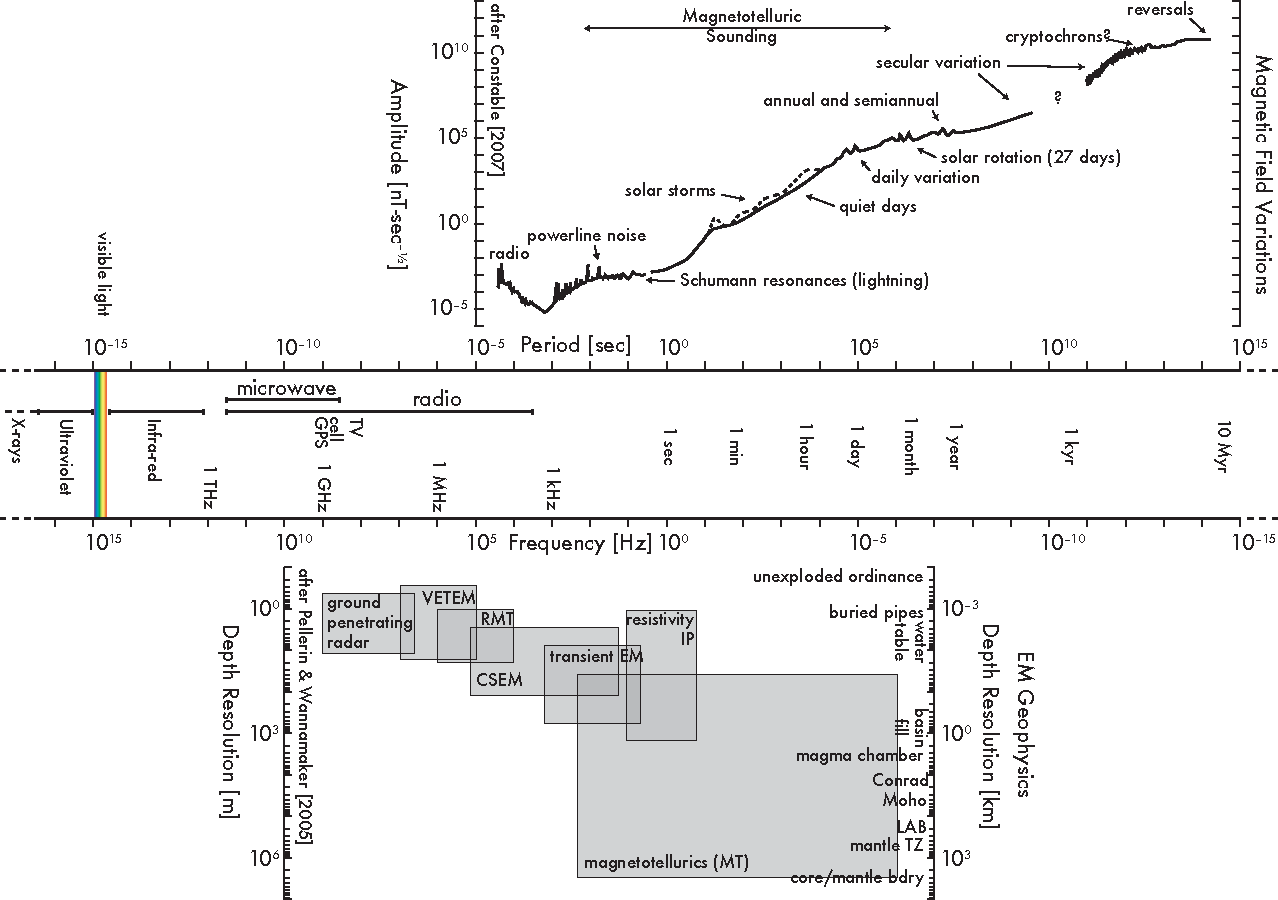
\includegraphics[angle=90]{electromagnetics/figures/EM_spectrum.pdf}
  }
  \caption{Electromagnetic spectrum utilized in geophysics.  Also shown is the
  source field for magnetotellurics (MT) and the depth resolution of each
  technique.  Abbreviations: VETEM, very-early time electromagnetics; CSEM,
  controlled-source electromagnetics; and IP, induced polarization.}
  \label{fig:spectrum}
\end{figure}

The electrical methods that you learned about in the previous few lectures are
also governed by Maxwell's equations utilizing Gauss's law of electricity which
only depends upon the electric field variations.  Now we'll be focusing on
techniques which include both the electric and magnetic field variations.  These
techniques fall into three categories:
\begin{description}
    \item[time domain,] techniques in which an applied electric field (by us)
    creates a time varying magnetic field;
    \item[frequency domain,] techniques in which time varying electric and
    magnetic fields, either natural or applied, result in time varying electric
    and magnetic fields.  Processing for these techniques are done in the
    frequency domain to simplify the mathematics;
    \item[ground-penetrating radar,] high frequency EM radiation is applied to
    the subsurface.
\end{description}

\section{Ground Penetrating Radar, GPR}
We won't spend much time on ground penetrating radar because the physics is
governed by the wave equation and as a result the techniques are in many ways
the same as seismic methods.

\section{Time-Domain Electromagnetics, TEM or TDEM}
\subsection{Magnetic induction}
The magnetic flux, $\Phi_{B}$, through a loop of wire (or body of rock) is
related to the magnetic field, $B$, by
\begin{equation*}
    \dv{\Phi_{B}}{t} = \dv{}{t} \fint{S}{} \vb{B}(t) \cdot \dd{\vb{A}}.
\end{equation*}
Hence, the $\Phi_{B}$ is the temporal change in the magnetic field through a
given area.  Assuming our loop is stationary, the magnetic flux is
\begin{equation*}
    \dv{\Phi_{B}}{t} = \fint{S}{} \dv{\vb{B}}{t} \cdot \dd{\vb{A}}.
\end{equation*}
Faraday's law tells us that a changing magnetic field within a conductive media
results in an electric field,
\begin{equation}
    \dv{\Phi_{B}}{t} = 
    \dv{}{t} \fint{S}{} \vb{B} \cdot \dd{\vb{A}} =
    -\cint{C} \vb{E} \cdot \dd{\vb{\ell}}.
    \label{eq-flux}
\end{equation}

The electromotive force (EMF), $\mathcal{E}$, is an induced voltage defined as
the energy per unit charge that travels around a loop, which we get from the
Lorentz force,
\begin{equation}
    \mathcal{E} = \cint{C} (\vb{E} + \vb{v} \times \vb{B}) \cdot
        \dd{\vb{\ell}}.
    \label{eq-emf}
\end{equation}
Again the second term on the right-hand side drops out since our loop is not
moving (i.e.\ $\vb{v} = 0$).  Therefore, from Equations \ref{eq-flux} and
\ref{eq-emf} we see that the a change in the magnetic flux (field) induces in a
EMF,
\begin{equation}
    \mathcal{E} = - \dv{\Phi_{B}}{t}.
\end{equation}

In time-domain electromagnetic, we measure this induced voltage to tell us about
the properties of the subsurface of the Earth.

\subsection{Conceptual model}
We make TEM measurements by using two loops, one which initiates the change in
magnetic flux (transmitter) and one which records the Earth's response
(receiver).  The current flowing through a transmitter is rapidly shut off,
resulting in change in the magnetic flux in the subsurface.  This change if flux
generates eddy currents which oppose the change in flux and create a
secondary magnetic field (Figure~\ref{fig:induction}).  This secondary magnetic
field decays away with time with characteristics related to the physical
properties of the body.  The decay in the secondary magnetic field generates a
change in magnetic flux in the receiver loop which generates a current that is
then measured.
\begin{figure}[hbt]
  \centerline{
    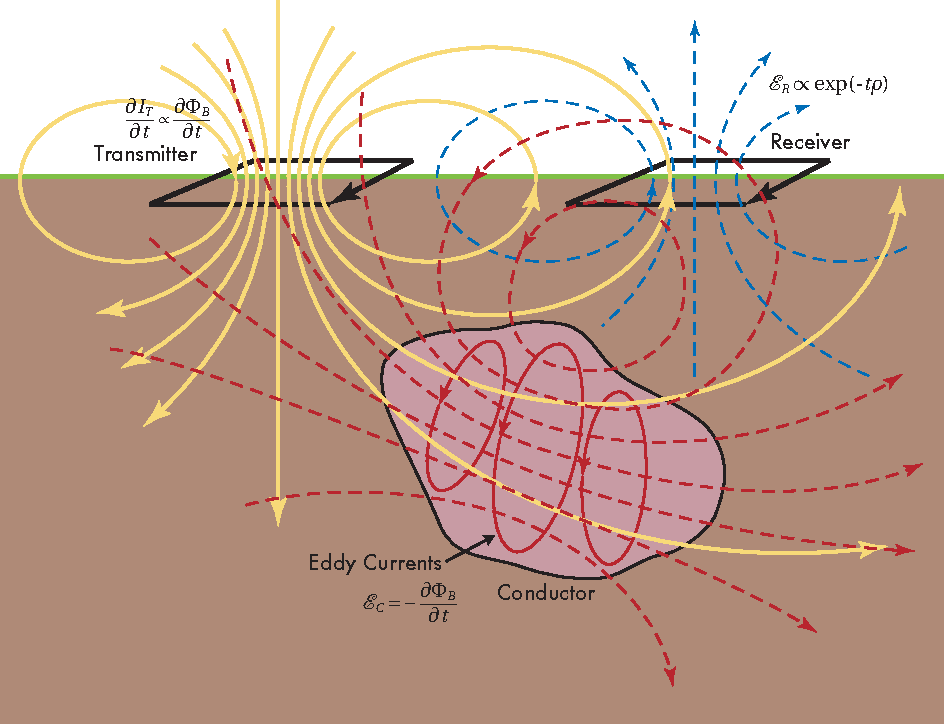
\includegraphics[]{electromagnetics/figures/induced_field.pdf}
  }
  \caption{The magnetic field of the transmitter (yellow) dissipates when it is
  switched off, inducing a current in the subsurface (solid red) generating a
  secondary magnetic field (red).  This secondary magnetic field decays
  generating a current in the receiver wire.}
  \label{fig:induction}
\end{figure}

The transmitter signal is generated by a set of alternating trapezoidal shaped
variations in current (Figure~\ref{fig:response}).  Ideally the shape would be a
square wave so that the change in flux do the transmitter is instantaneous but,
in reality, self-inductance within the loop prevents such a rapid turn-off.
Measurements are not taken during the turn-off, but are recorded during the off
time after a brief delay ($\sim\mu$s).  The response in the receiver due to the
changing Earth fields are recorded in the receiver in time gates which average
the induced voltage over a short time interval to reduce the influence of noise.
The time gates are typically recorded in a logarithmic separation in time.
\begin{figure}[hbt]
  \centerline{
    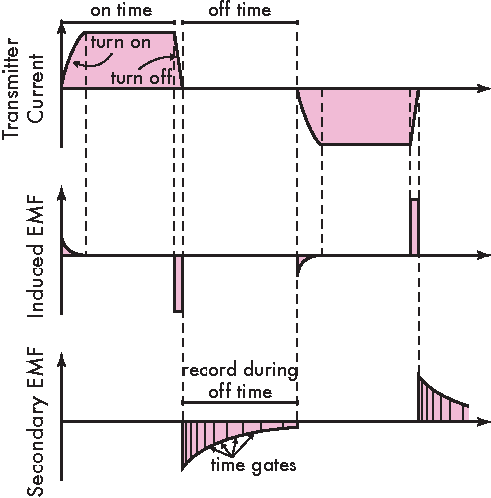
\includegraphics[]{electromagnetics/figures/induced_response.pdf}
  }
  \caption{Transient electromagnetic transmitter and receiver signals.}
  \label{fig:response}
\end{figure}

The instant the transmitter is turned off, an image current is created within
the Earth that opposes the change in the magnetic field ($t \sim 0$).  As the
induced magnetic field changes, it induces additional currents which travel
further into the Earth.  This spreading with time continues outward and
downwards with time ($t_{1}, t_{2} > 0$).  For an ideal half-space this
spreading occurs at 30$^\circ$ (Figure~\ref{fig:smoke}).  Therefore, the time
after the transmitter is turned off can be related to depth (and/or distance to
the receiver if not an in-loop configuration see below).  The field also
attenuates with time until it can no longer be resolved over ambient
(environmental and instrument) noise levels.
\begin{figure}[hbtp]
  \centerline{
    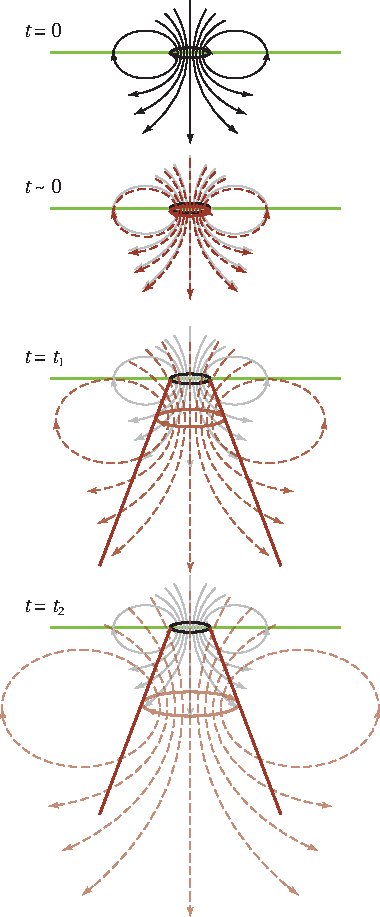
\includegraphics[]{electromagnetics/figures/smoke_rings.pdf}
  }
  \caption{Induction, spreading, and attenuation of electrical currents within
  the Earth following a change in the transmitter current.}
  \label{fig:smoke}
\end{figure}


\subsection{Circuit analogy}
The math behind electromagnetic induction in the Earth can be quite complicated
so we'll look at a simplified analogy \citep{Grant&West1965}.  The currents
induced in a conductive body can be thought of in terms of a circuit.  The
simplified circuit has an induced voltage due to the transmitter, a resistance
to the flow of current, and an inductance that resists the change in magnetic
flux through the body (Figure~\ref{fig:analogy}).  While this greatly simplifies
the actual physics, it is instructive understanding for understanding some of
the general characteristics of the true TEM method and the response to differing
properties of the subsurface.
\begin{figure}[hbtp]
  \centerline{
    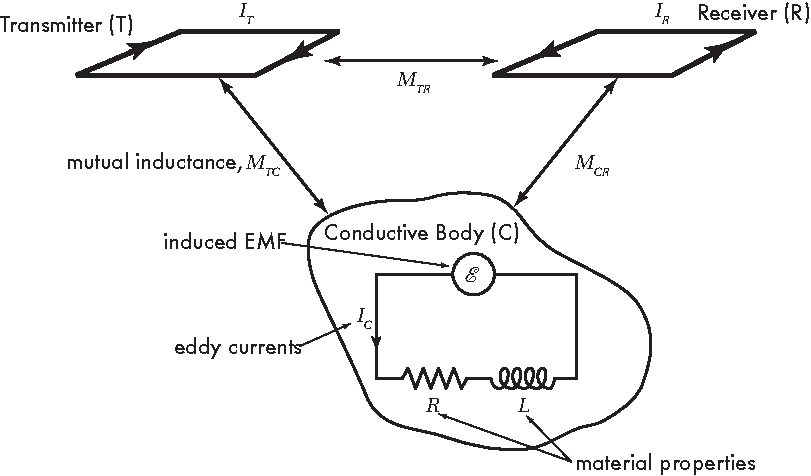
\includegraphics[]{electromagnetics/figures/circuit_analogy_bw.pdf}
  }
  \caption{A simplified view of electromagnetic induction in the Earth.}
  \label{fig:analogy}
\end{figure}

The voltage around a closed loop is zero according to Kirchoff's second law,
\begin{equation*}
    \mathcal{E} - V_{L} - V_{R} = 0.
\end{equation*}
The voltage of a resistor is given by $V_{R} = I_{\mathrm{C}}(t) R$, for an
inductor the voltage drop is $V_{L} = L \dd{I_{\mathrm{C}}(t)}\dd{t}$, where
$I_{\mathrm{C}}$ is the current flowing through the body.  The EMF coupling between
the transmitter and anomalous body is an inductive effect related to the change
in current of the transmitter.  We can write the induced voltage term as
$\mathcal{E} = - M_{\mathrm{TC}} \dv{}{t} I_{\mathrm{T}}$, where $I_{\mathrm{T}}$ is the
transmitter current. The coupling between the transmitter and conductive body
within the Earth is given by $M_{\mathrm{TC}}$ and has units of inductance.  It is
effectively a mutual inductance that depends upon the shape and size and
orientations of the transmitter loop and the conductive body as well as the
distance between the two and the conductivity of the conductive body.  Thus, we
can complete our loop,
\begin{equation}
    -M_{\mathrm{TC}} \dv{}{t}I_{\mathrm{T}}(t) - \left( L \dv{}{t}
    I_{\mathrm{C}}(t) + R I_{\mathrm{C}}(t) \right) = 0.
\end{equation}
The transmitter current is represented by a ramp function occurring over a short
time interval $\Delta t$, such that $I_{\mathrm{T}} = I_0 u(t)$ where
\begin{equation*}
    u(t) = 
    \begin{cases}
        0 & \text{if $t < 0$}, \\
        t\, \Delta t^{-1} & \text{if $0 \leq t \leq \Delta t$}, \\
        1 & \text{if $t > \Delta t$}.
    \end{cases}
\end{equation*}
\begin{figure}[hbt]
  \centerline{
    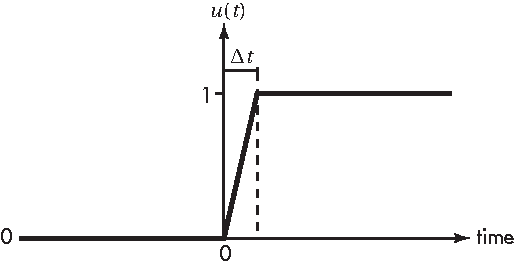
\includegraphics[]{electromagnetics/figures/u.pdf}
  }
  \caption{Normalized transmitter current, u(t). Ideally we try to make turn-on
  (-off) time, $\Delta t$, as small as possible.}
  \label{fig:u}
\end{figure}

We can rewrite the circuit voltages as
\begin{equation}
    \left( L \dv{}{t} + R \right) I_{\mathrm{C}} = 
        - M_{\mathrm{TC}} I_{0} \dv{u(t)}{t}.
    \label{eq-Ic}
\end{equation}
So lets now explore the three cases of $u(t)$.
\begin{enumerate}
    \item {\bf Before switching on the current, $t < 0$ and $u(t) = 0$.}

    This results in the trivial steady-state solution, $I_{\mathrm{C}} = 0$.

    \item {\bf As the transmitter current is turned off, $0 \leq t \leq \Delta
    t$ and $u(t) = t\, \Delta t^{-1}$.}

    The transmitter current,
    \begin{equation*}
        I_{\mathrm{T}} = I_{0} \dv{}{t} \left[ t\, \Delta t^{-1} \right] =
            I_{0}\, \Delta t^{-1},
    \end{equation*}
    when combined with Equation \ref{eq-Ic} gives
    \begin{equation*}
        \left(L \dv{}{t} + R \right) I_{\mathrm{C}}(t) 
            = - \frac{M_{\mathrm{TC}} I_0}{\Delta t}.
    \end{equation*}
    This is simply the differential equation $a_{0} \dd{y(x)}/\dd{x} + a_{1} y(x)
    = c$, with the initial condition $y(0) = y_{0}$, which has the solution $y =
    y_{0} \exp(-x a_{1}/a_{0}) + c/a_{0}$.  Using the coefficients from our ODE
    and knowing that $I_{\mathrm{C}} = 0$ at $t = 0$, we find
    \begin{equation*}
        I_{\mathrm{C}}(t) = - \frac{M_{\mathrm{TC}} I_0}{R\, \Delta t}
            \left[ 1 - \exp \left( -t \frac{R}{L} \right) \right].
    \end{equation*}
    We can simplify this expression further by using a Taylor series
    approximation for $\exp(-x) = 1 - x + \frac{1}{2}x^2 - \ldots$, which we will
    truncate after the first term.  This approximation introduces a small error
    only when $x \ll 1$, or in our case when $t \ll L/R$.  Therefore, the
    current induced in the Earth as the transmitter is turned off is
    \begin{equation}
        I_{\mathrm{C}}(t) \approx - \frac{M_{\mathrm{TC}} I_0}{L\, \Delta t} t.
    \end{equation}
    Since we will also need the initial current condition in for the third case,
    we can show that as long as our transmitter current is turned off
    sufficiently fast, $\Delta t \ll L/R$, the induced current at $t = \Delta t$
    is $I_{\mathrm{C}} = - M_{\mathrm{TC}} I_0 L^{-1}$.

    \item {\bf When the transmitter off, $t > \Delta t$ and $u(t) = 1$.}
    
    Since $\dd{u}/\dd{t} = 0$ in this case, from Equation~\ref{eq-Ic} we find
    \begin{equation*}
        \left( L \dv{}{t} + R \right) I_{\mathrm{C}} = 0.
    \end{equation*}
    This ODE is very similar to the previous one we encountered.  The solution
    of which is similar.  The solution to $a_{0} \dd{y}/\dd{x} + a_{1} y = 0$ is
    $y = k \exp (-t a_{1}/a_{0})$.  Again we input our coefficients from the
    above ODE and our final condition to the previous time interval (now our
    initial condition) to give us our estimated current in the conductive body,
    \begin{equation}
        I_{\mathrm{C}} \approx - \frac{M_{\mathrm{TC}} I_0}{L}
            \exp \left( -t \frac{R}{L} \right) .
    \end{equation}
\end{enumerate}

A similar circuit analogy may be drawn to examine the response in the receiver
loop, but I will leave that derivation as an exercise in class as well.

\begin{framed}
    {\bf Aside:} Consider the second and third cases above.  What is the induced
    current most sensitive to?  What changes as you transition from the
    early-time (case 2) to the late-time (case 3)?

    How does the value of R/L affect the rate of decay of the
    current?
\end{framed}


\subsection{TEM survey}
Transient electromagnetic measurements are conducted using two loops.  The loops
may be any shape, but typically square and nearly circular are chosen because
they simplify the math.  One loop inducing a current within the Earth
(transmitter, T) and a second which receives the Earth's response (receiver, R).
If the Earth were homogeneous or layered vertically, we would only need to
measure the vertical component.  Surveys can measure only one component of the
subsurface (usually depth), but it is not uncommon for horizontal components to
be measured as well because of their sensitivity to vertical structures.
Possible transmitter receiver pairs are shown in Figure~\ref{fig:pairs}.
\begin{figure}[hbt]
  \centerline{
    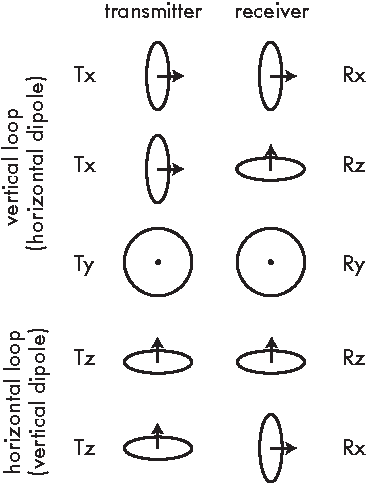
\includegraphics[]{electromagnetics/figures/tr_pairs.pdf}
  }
  \caption{Transmitter (T) and receiver (R) pair orientations.}
  \label{fig:pairs}
\end{figure}

The layout geometry may also vary again each with their own advantages and
disadvantages.  Three common variations are shown in Figure~\ref{fig:geometry}.
\begin{figure}[hbt]
  \centerline{
    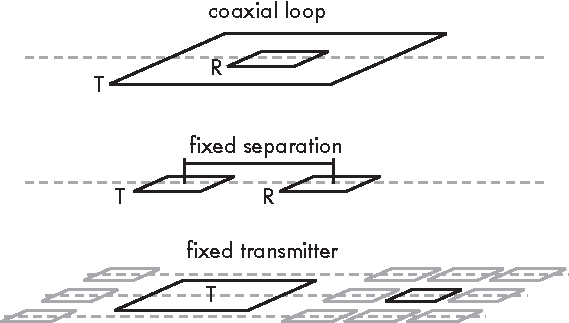
\includegraphics[]{electromagnetics/figures/tr_geometry.pdf}
  }
  \caption{Field layout geometries.}
  \label{fig:geometry}
\end{figure}
\begin{description}
    \item[Coaxial] - the receiver loop has a coincident center with the
    transmitter loop.\\
        \begin{itemize}
            \item Pros: convenient; strong signal; no blind zones 
            \item Cons: complex anomaly shape
        \end{itemize}
    \item[Fixed separation] - the transmitter and receiver loops are always the
    same distance apart.  This is the preferred method for many portable
    systems (e.g.\ aircraft, cart, hand-carry). \\
        \begin{itemize}
            \item Pros: less confusing anomaly shape
            \item Cons: weaker signals; less convenient (unless the loops are
            mounted to a movable platform)
        \end{itemize}
    \item[Fixed transmitter] - the transmitter remains in a static location
    while the receiver is placed in multiple positions. This method is often
    employed with greater depth of penetration so that a large transmitter
    moment can be employed.\\
        \begin{itemize}
            \item Pros: reduced rate of fall-off; constant source field
            \item Cons: blind zones; dependent on location of transmitter
        \end{itemize}
\end{description}

The strength of the induced voltage and receiver sensitivity are dependent upon
their magnetic moment.  If you will recall from magnetics, the magnetic moment
has units of A~m$^{2}$, which is simply a current times an area.  Therefore, for
a loop of wire with current, $I$, and area, $A$, the moment is $m = I A$.  We
can actually increase the moment by making multiple loops (or turns).  For $N$
turns of wire, the magnetic moment is $m = N I A$.

For a receiver, we typically want many turns to increase the sensitivity, but
for a transmitter, we often use only one turn and increase the current instead.
The inductance is proportional to the area and number of turns by, $L
\propto N^{2} A$.  Since the definition of inductance is related to the
magnetic flux by $\Phi_{B} = L I N^{-1}$, the greater the number of turns
the larger the flux.  The reason for a single loop transmitter is because we
want the magnetic field it generates to decay as rapidly as possible once
we switch it off.

\subsection{Sensitivity and skin depth}

The depth at which the induced magnetic field reaches a maximum is related to
the time after the current is shut off by
\begin{equation*}
    z = \left( \frac{2 t}{\sigma \mu} \right)^{1/2}.
\end{equation*}
However in reality, the depth of sensitivity is smaller by a factor of $\sim$2.

\section{Frequency-domain}
Loop-loop systems can also be used to record time data that is processed in the
frequency domain.  But I will not discuss these here.  Instead, I am going to
focus on a deeper technique.  One that is used for the study of basin structure
and hydrology, geothermal systems, and imaging the lithosphere and upper mantle. 

These solutions are for $E$ and $H$ in time and space, where $\vb{E} =
\vb{E}(x,y,z,t)$ and $\vb{H} = \vb{H}(x,y,z,t)$.

\subsection{Magnetotellurics}

\subsubsection{Helmholtz equation}
The diffusion equations in $E$ and $H$ (Equation~\ref{eq-diffusion}) are
\begin{align*}
    \nabla^2 \vb{E} = \mu \sigma \pdv{\vb{E}}{t} \\
    \nabla^2 \vb{H} = \mu \sigma \pdv{\vb{H}}{t}.
\end{align*}
The Fourier transform $\vb{E}(x,y,z,t)
\overset{\mathcal{F}}{\longleftrightarrow} \vb{E}(x,y,z,\omega)$ with $e^{i
\omega t}$ time dependence results in the Helmholtz equation,
\begin{align*}
    \nabla^2 \vb{E} + k^2 \vb{E} & = 0 \\
    \nabla^2 \vb{H} + k^2 \vb{H} & = 0, \\
\end{align*}
where $k = (1 - i) \left( \frac{\sigma \mu}{\omega} \right)$.  Note $i$ here is
referred to as the complex number, $i = (-1)^{1/2}$ (Appendix~\ref{apx:complex}
discusses complex numbers in greater detail.  The solution to the Helmholtz
equation requires additional Fourier transforms in space ($\vb{E}(x,y,z,\omega)
\overset{\mathcal{F}}{\longleftrightarrow} \vb{E}(k_x,k_y,\omega)$) to arrive at a
solution,
\begin{equation}
    \vb{E} = \underbrace{E^{(+)}(k_x,k_y,\omega) e^{i k_z z}}_{\mathrm{upgoing}}
        + \underbrace{E^{(-)}(k_x,k_y,\omega) e^{-i k_z z}}_{\mathrm{downgoing}}, 
\end{equation}
where $k_z = \left(k^2 - k_x^2 - k_y^2\right)^{1/2}$ and $E^{(+)}$ and $E^{(-)}$
are the coefficients for an upgoing and downgoing propagating fields,
respectively.  Since the $E$ and $H$ fields must vanish as $z \to \infty$ (down
into the Earth), $E^{(+)} = 0$.

\subsubsection{One-dimensional theory}
We make a number of assumptions for the 1-D case:
\begin{enumerate}
    \item the quasi-static approximation is valid; 
    \item the waves incident to the surface are planar and vertical;
    \item variations in $\mu$ and $\epsilon$ are small relative to variations in
    the conductivity and we can therefore assume the free-space values; and
    \item resistivity varies only as a function of depth, $\rho(z)$.
\end{enumerate}
The second assumption implies that $k_{x} = k_{y} = 0$ and $k_{z} = \pm k$,
where
\begin{equation}
    k = (1 - i) \sqrt{\frac{\sigma \mu_0 \omega}{2}}
\end{equation}
(Note that $k$ has real and imaginary parts).
In the 1-D solution the fields are orthogonal (i.e.\ $\vb{E} \cdot \vb{H} =
0$).  Since, $E$ and $H$ are orthogonal, we can assume $\vb{E} = E\hat{x}$ and
$\vb{H} = H\hat{y}$.  Hence we can write the fields
\begin{align}
    E_x & = E_0 e^{-(1 + i) \sqrt{\frac{\sigma \mu_0 \omega}{2}} z} \\
    H_y & = H_0 e^{-(1 + i) \sqrt{\frac{\sigma \mu_0 \omega}{2}} z}.
\end{align}

\subsubsection{Skin-depth}
Much as we have a diffusion length for TEM, we can define a skin depth as the
depth at which the fields reduce to $e^{-1}$ of their initial
magnitude.  However, the expression for our field includes the complex quantity
$k$.  We break $k$ into a real and imaginary part, $k = k_R - i k_I$, where $k_R
= \Re(k)$ and $k_I = |\Im(k)|$, respectively.  Doing so allows us to write the
electric field as
\begin{align*}
    E &= E_0 e^{-i(k_R - i k_I)z} \\
    &= E_0 e^{-k_I z} e^{-i k_R z} .
\end{align*}
Writing the electric field in the above form allows us to see that the electric
field is exponentially decreasing with depth.  Note $k_I$ is real valued with
units, length$^{-1}$.  Therefore, $k_I^{-1}$ is a characteristic depth constant,
which we call the skin depth,
\begin{align}
    \delta &= k_I^{-1} \\
    &= \left( \frac{2}{\sigma \mu_0 \omega} \right)^{1/2}.
\end{align}

\begin{framed}
The wavelength, $\lambda$, of a wave traveling through a medium is related to
the wavenumber, $k$, by
\begin{equation*}
    \lambda = 2 \pi |k|^{-1}.
\end{equation*}
The wavelength is related to the skin depth by 
\begin{equation*}
    \lambda = 2 \pi \delta ,
\end{equation*}
which allows us to write the wavelength in terms of the frequency as
\begin{equation*}
    \lambda = 2 \left( \frac{\pi \rho \tau}{\mu_0} \right)^{1/2},
\end{equation*}
recalling that $\omega = 2\pi f = 2\pi \tau^{-1}$ where $\tau$ is the period of
the wave.

The velocity of a wave can be determined by its frequency and wavelength,
\begin{equation*}
    v = \lambda f .
\end{equation*}
The phase velocity of an electromagnetic wave traveling through a medium are
related by
\begin{align*}
      v &= 2 \pi \delta \frac{\omega}{2 \pi}\\
      &= \delta \omega \\
      &= \left( \frac{2 \omega}{\sigma \mu_0} \right)^{1/2}.
\end{align*}
Note: the velocity of an electromagnetic wave is related to the conductivity of
the material (i.e., the speed of light is not constant outside of a vacuum).
\end{framed}


\subsubsection{Impedance, phase and resistivity}
{\bf Impedance} is a complex resistivity and has a frequency dependence.  We define
the impedance as
\begin{equation}
    Z = \frac{E_x(\omega)}{H_y(\omega)}.
\end{equation}
We can derive the characteristic impedance of a region then by using our
solutions to the Helmholtz equation and Faraday's law,
\begin{equation*}
    -\mu_0 \pdv{}{t} \vb{H} = \curl \vb{E}.
\end{equation*}
In the Fourier domain this equation is just
\begin{align*}
    -\mu_0 (H_y) & = \pdv{}{z} E_x \\
    -\mu_0 (H_y) & = -\frac{1}{i \omega} \pdv{}{z} \left( E_0 e^{-ikz} \right) \\
    H_y & = \frac{k}{\omega \mu_0} E_0 e^{-ikz}.
\end{align*}
Therefore,
\begin{align}
    Z & = \frac{E_{x}}{\frac{k}{\omega \mu_0}E_x} \\
    Z & = \frac{\omega \mu_0}{k}.
\end{align}

\begin{framed}
    {\bf Aside:} Free space (vacuum) also has an impedance, although $\sigma =
    0$ for free-space so we do not take the quasi-static approximation.  The
    impedance of free space is therefore defined in terms of the fundamental
    constants
    \begin{equation*}
        Z_{0} = \sqrt{\frac{\mu_0}{\epsilon_0}} \approx 376.7\; \Omega. 
    \end{equation*}
    However, do not confuse this with the resistivity of air which is on the
    order of 10$^{16}$~$\Omega$~m$^{-1}$.
\end{framed}

{\bf Resistivity} of a body is related to the conductivity by $\rho =
\sigma^{-1}$.  The goal of our magnetotelluric survey is to determine the
resistivity structure of the Earth.  We can can relate the resistivity to the
impedance above by using the definition of $k$
\begin{align*}
    Z & = \omega \mu_0 (1 + i) \left(\frac{\rho}{ 2 \omega \mu_0} \right)^{1/2} \\
      & = (1 + i) \left( \frac{\omega \mu_0 \rho}{2} \right)^{1/2}.
\end{align*}
Solving the above result for $\rho$,
\begin{equation*}
    \rho = -\frac{i}{\omega \mu_0} Z^2.
\end{equation*}
Note that this result for $\rho$ is a complex quantity.  We can choose to have a
real valued resistivity which we define as
\begin{equation*}
    \rho = \frac{1}{\omega \mu_0} | Z |^2.
\end{equation*}
For an impedance measured at the surface of the Earth, we call this the apparent
resistivity, designated by $\rho_a$, and relate it to the fields we measure at
the surface by
\begin{align*}
    \rho_a & = \frac{1}{\omega \mu_0} | Z_S |^2 \\
           & = \frac{1}{\omega \mu_0} \left| \frac{E_x}{H_y} \right|^2.
\end{align*}

{\bf Phase} is related to the imaginary part of the impedance by
\begin{equation*}
    Z = |Z| e^{i \phi}
\end{equation*}
(see Appendix~\ref{apx:complex} for a discussion of complex numbers).  We can
determine the phase by
\begin{equation*}
    \phi = \tan^{-1} \left( \frac{\Im (Z)}{\Re (Z)} \right).
\end{equation*}
While we perform our calculations in radians, we often discuss or plot the phase
in degrees.  The phase is related to the apparent resistivity by
\begin{equation*}
    \phi(\Log \omega) = \frac{\pi}{4}
        \left( 1 + \dv{(\Log \rho_a)}{(\Log \omega)} \right),
\end{equation*}
where $\Log$ is $\log_{10}$.  Therefore when the resistivity is not changing,
$\dv{(\Log \rho_a)}{(\Log \omega)} = 0$, $\phi = \pi/4$ or 45$^\circ$.


\subsubsection{Half-space model}
Now that we have defined the impedance, we would like to estimate the impedance
at the surface of the Earth, $Z_s$.  We will start with the solution for a
half-space and then build upon that to derive the solution for an arbitrary
number of horizontal layers.

The initial waves coming from above strike the Earth's surface.  Most of the
energy is reflected back into space, while a small amount is transmitted into
the Earth.  Consider three fields at the surface, the incident field, the
reflected field and the transmitted field,
\begin{align}
    \text{incident wave:} &
    \begin{cases}
        E^i_x = E^i_0 e^{-i k_0 z}, \\
        H^i_y = H^i_0 e^{-i k_0 z};
    \end{cases} \\
    \text{reflected wave:} &
    \begin{cases}
        E^r_x = E^r_0 e^{i k_0 z}, \\
        H^r_y = H^r_0 e^{i k_0 z};
    \end{cases} \\
    \text{transmitted wave:} &
    \begin{cases}
        E^t_x = E^t_1 e^{-i k_1 z}, \\
        H^t_y = H^t_1 e^{-i k_1 z}.
    \end{cases}
    \label{eq-sfield}
\end{align}
Note the sign difference for the reflected wave which denotes the field is
traveling away from the center of the Earth while the other travel towards.
Continuity of $E$ and $H$ at $z = 0$ requires
\begin{align*}
    E^i_x + E^r_x & = E^t_x, \\
    H^i_y + H^r_y & = H^t_y.
\end{align*}
Recall that impedance is given by $Z = E/H$, which allows us to write
the above equations in terms of $E$'s,
\begin{align*}
    E^i_x + E^r_x & = E^t_x, \\
    \frac{E^i_x}{Z_0} - \frac{E^r_x}{Z_0} & = \frac{E^t_x}{Z_1},
\end{align*}
where $Z_0$ and $Z_1$ are the characteristic impedances of the air and
half-space respectively.  We can solve each of these in terms of $E^i_0$,
\begin{align*}
    E^t_x = \frac{2 Z_1}{Z_0 + Z_1} E^i_x, \\
    E^r_x = \frac{Z_1 - Z_0}{Z_0 + Z_1} E^i_x.
\end{align*}
The impedance ratios above are called the transmission and reflection
coefficients, respectively.

The surface impedance is defined in terms of the total $E$ and $H$ fields at $z
= 0$, which we get from either side of Equation~\ref{eq-sfield}.  Taking then 
\begin{align*}
    Z_s & = \lim_{z \to 0} \frac{E^t_x}{H^t_y}, \\
        & = \lim_{z \to 0}
        \left[ \frac{2 Z_1}{Z_0 + Z_1} E^i_0 e^{-i k_0 z} \right]
        \left[ \left( \frac{2 Z_1}{Z_0 + Z_1} \right)
        \left( \frac{E^i_0 e^{-i k_0 z}}{Z_1} \right) \right]^{-1} \\
        & = \left[ \frac{2 Z_1}{Z_0 + Z_1} \right]
        \left[ \frac{2 Z_1}{Z_0 + Z_1} \frac{1}{Z_1} \right]^{-1} \\
        & = Z_1.
\end{align*}
Had we taken the other side of Equation~\ref{eq-sfield} we would obtain the same
result.

\subsubsection{Layered model}
For a layered model we can solve for the impedance at each layer interface very
similar to the half-space model solution by writing equations for the incident,
reflected, and transmitted waves at each interface.  The system of equations for
$N$ layers becomes $2N$.  There is another way, which allows us to circumvent
the additional equations and the method we will apply here.

The ultimate goal of this derivation is to derive a relationship for the surface
impedance as a function of frequency (angular frequency to be exact).  Why do we
just care about the surface impedance and not the impedance of each layer?  It
is because we cannot measure the impedance of each layer directly, only the
impedance at the surface.  We'll also use this relationship to develop a few
generalities that are incredibly insightful into the efficacy of the method to
provide insight about the physical properties of the Earth (specifically
conductivity/resistivity) and their dimension.

Consider a simplified model of the Earth with $N$ flat layers with differing
conductivities and thicknesses overlying a half-space with constant
conductivity.
\begin{figure}[hbt]
  \centerline{
    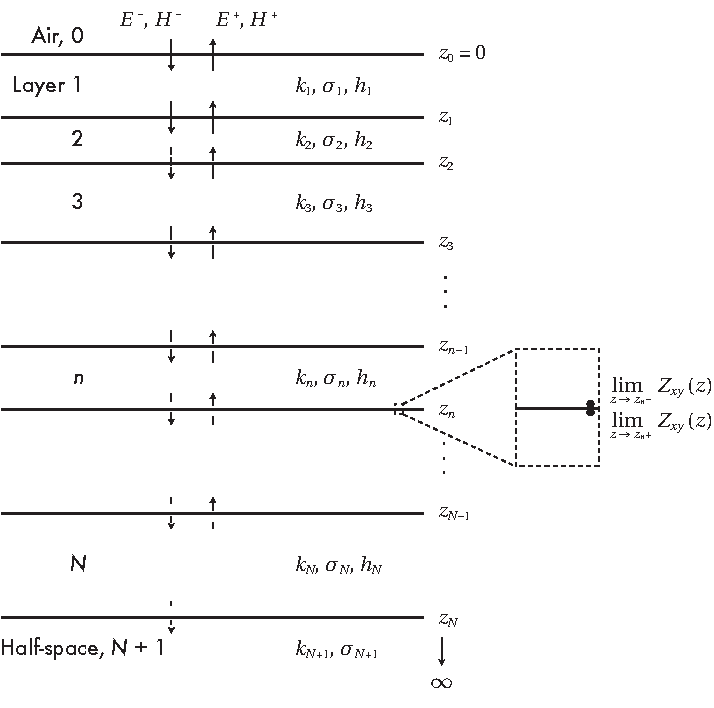
\includegraphics[]{electromagnetics/figures/EM_layers.pdf}
  }
  \caption{$N$-layered Earth over a half-space.}
  \label{fig:nlayers}
\end{figure}
For any layer, $n = [0,1,2,\cdots,N,N+1]$, there is a horizontal magnetic field
downgoing component (transmitted from above) and an upgoing component (reflected
from below),
\begin{align}
    E_{x}(z,\omega) & = E^{+}_{x,n} e^{+i k_{n} z} + E^{-}_{x,n} e^{-i k_{n} z} \\
    E_{y}(z,\omega) & = \underbrace{E^{+}_{y,n} e^{+i k_{n} z}}_{\mathrm{reflected}} +
    \underbrace{E^{-}_{y,n} e^{-i k_{n} z}}_{\mathrm{transmitted}}
    \label{eq:elayer}
\end{align}
(Figure \ref{fig:nlayers}).  For the half-space solution we also assumed that
there was only one component of the electric field.  However, for a more general
plane wave we have to consider $E$ and $H$ fields in both the $x$ and $y$
directions.  Recall in the frequency domain $\curl \vb{E} = i \omega \mu_0
\vb{H}.$  If we write this in the determinant notation (see
Appendix~\ref{apx:vcalc})
\begin{equation*}
    \curl \vb{E} (z,\omega) =
    \begin{vmatrix}
        \hat{x} & \hat{y} & \hat{z} \\
        0 & 0 & \pdv{}{z} \\
        E_{x} & E_{y} & 0
    \end{vmatrix}
    = i \omega \mu_0 (H_x \hat{x} + H_y \hat{y}),
\end{equation*}
note only derivatives in the $z$ direction are necessary because our field is
vertically incident and therefore the derivatives in the $x$ and $y$ dimensions
cancel.  Now performing the curl we find
\begin{align*}
    H_x & = -\frac{1}{i \omega \mu_0} \dv{E_y}{x} \\
    H_y & = \frac{1}{i \omega \mu_0} \dv{E_x}{y}.
\end{align*}
Now we take the derivative of the electric field within each layer,
\begin{align}
    H_x(z,\omega) & = - \frac{k_n}{\omega \mu_0} (E^{+}_{y,n} e^{+i k_{n} z} -
        E^{-}_{y,n} e^{-i k_{n} z}) \\
    H_y(z,\omega) & = \frac{k_n}{\omega \mu_0} (E^{+}_{x,n} e^{+i k_{n} z} -
        E^{-}_{x,n} e^{-i k_{n} z}).
    \label{eq:hlayer}
\end{align}
Previously, we defined the characteristic impedance of a layer as the ratio of
the electric to the magnetic fields (i.e.\ $Z = E/H$).  Because we have field
components in two orthogonal directions we can define two components of the
impedance,
\begin{align*}
    Z_{xy}(z,\omega) & = \frac{E_{x}(z,\omega)}{H_{y}(z,\omega)} \\
    Z_{yx}(z,\omega) & = -\frac{E_{y}(z,\omega)}{H_{x}(z,\omega)}.
\end{align*}
Inputting our results for the fields (Equations \ref{eq:elayer} and
\ref{eq:hlayer}) we find
\begin{equation*}
    Z_{xy}(z,\omega) = \frac{\omega \mu_0}{k_n}
        \frac{E^{+}_{x,n} e^{+i k_{n} z} + E^{-}_{x,n} e^{-i k_{n} z}}
        {E^{+}_{x,n} e^{+i k_{n} z} - E^{-}_{x,n} e^{-i k_{n} z}}.
\end{equation*}

In order to simplify our problem somewhat we are going to make two substitutions
that allow us to reduce our system of equations to a single unknown per layer
related to the ratio of the upgoing and downgoing electric fields rather each
individually.   The first will be to multiply by $(E_x^+ E_x^-)^{-1/2}/(E_x^+
E_x^-)^{-1/2}$, which is the equivalent to multiplying by 1.  This allows us to
write our impedances as the ratio of the magnitudes of the upgoing and downgoing
waves,
\begin{equation*}
    Z_{xy}(z,\omega) = \frac{\omega \mu_0}{k_n}
        \frac{(E^{+}_{x,n}/E^{-}_{x,n})^{1/2} e^{+i k_{n} z} 
            + (E^{-}_{x,n}/E^{+}_{x,n})^{1/2} e^{-i k_{n} z}}
        {(E^{+}_{x,n}/E^{-}_{x,n})^{1/2} e^{+i k_{n} z} 
            - (E^{-}_{x,n}/E^{+}_{x,n})^{1/2} e^{-i k_{n} z}}.
\end{equation*}
The next substitution allows us to put the field ratios into the exponent using
the equivalent of $e^{\log(x)} = x$,
\begin{equation*}
    (E^{+}_{x,n}/E^{-}_{x,n})^{1/2} = e^{-r_n} =
    e^{-\log[(E^{+}_{x,n}/E^{-}_{x,n})^{1/2}]}
\end{equation*}
(I am using `$\log$' to denote the natural logarithm, which is also frequently
denoted as `$\ln$').  Applying this substitution, we have
\begin{equation*}
    Z_{xy}(z,\omega) = \frac{\omega \mu_0}{k_{n}}
        \frac{e^{i k_n z - r_n} + e^{-(i k_n z - r_n)}}
        {e^{i k_n z - r_n} - e^{-(i k_n z - r_n)}},
\end{equation*}
which is simply
\begin{equation}
    Z_{xy}(z,\omega) = \frac{\omega \mu_0}{k_{n}} \coth (i k_n z - r_n),
    \label{eq:Zn}
\end{equation}
for $z_{n} < z < z_n+1$ where $\coth$ is the hyperbolic cotangent (see
Appendix~\ref{apx:hyper}).  Now we have our layer impedance in terms of single
unknown, $r_{n}$.

The horizontal components of the electric and magnetic field are continuous
across a layer interface.  Therefore, the impedance on both sides of a boundary
($z = z_n$) must also be continuous.  Since there is a discontinuity at the
boundary, we cannot simply compute the impedance at the boundary, but can
compute the result as we approach very very very closely from either side, hence
\begin{equation*}
    \lim_{z \to z_n-} Z_{xy}(z,\omega) = \lim_{z \to z_n+} Z_{xy}(z,\omega),
\end{equation*}
where $z \to z_n-$ approaches from the layer above and $z \to z_n+$ approaches
from the layer below.  Inputting the Equation~\ref{eq:Zn} from above the
interface, we have
\begin{equation*}
    \frac{\omega \mu_0}{k_{n}} \coth (i k_n z_n - r_n)
        = \lim_{z \to z_n+} Z_{xy}(z,\omega).
\end{equation*}
Solving for $r_n$, we find
\begin{equation}
    r_n = i k_n z_n - \coth^{-1} 
        \left[ \frac{k_n}{\omega \mu_0} \lim_{z \to z_n+} Z_{xy}(z) \right].
\end{equation}
Next, to find the impedance at the previous interface, $n - 1$, we will stay
within layer $n$, and approach from below and use our result for $r_n$, which
gives
\begin{equation*}
    \lim_{z \to z_{n-1}+} Z_{xy}(z,\omega) = \frac{\omega \mu_0}{k_n} 
    \coth \left\{
        i k_n z_{n-1} - 
        \left[i k_n z_{n} - 
            \coth^{-1} \left(
                \frac{k_{n}}{\omega \mu_0} \lim_{z \to z_{n}+} Z_{xy}(z,\omega)
            \right)
        \right]
    \right\}
\end{equation*}
Rearranging somewhat we find a term $i k_n (z_{n-1} - z_n)$ which is the same as
$-i k_n h_n$, where $h_n$ is the thickness of the $n$-th layer.  This allows us
to write the impedance at the top of layer $n-1$ as
\begin{equation}
    \lim_{z \to z_{n-1}+} Z_{xy}(z,\omega) = 
        \frac{\omega \mu_0}{k_n}
        \coth \left[ -i k_n h_n + \coth^{-1} \left( \frac{k_n}{\omega \mu_0}
        \lim_{z \to z_{n}+} Z_{xy} (z,\omega) \right) \right].
    \label{eq:layersoln}
\end{equation}
We can use the identity, $\coth(a + \coth^{-1} b) \equiv \tanh(a + \tanh^{-1} b)$, to
write this result in the more common form.

However, below the last layer sits a half-space (i.e.\ no lower interface) and
as a result cannot include a reflected wave traveling up through the half-space.
Hence for the half-space,
\begin{align*}
    E_x(z,\omega) & = E_{x,N+1}^- e^{-i k_{N+1} z} \\
    H_y(z,\omega) & = \frac{k_{N+1}}{\omega \mu_0} E_{x,N+1}^- e^{-i k_{N+1} z} \\
    Z_{xy}(z,\omega) = \frac{E_{x,N+1}(z,\omega)}{H_{y,N+1}(z,\omega)} & 
        = \frac{\omega \mu_0}{k_{N+1}}, \\
\end{align*}
for $z_N < z \leq \infty$.  Just as we found for the non-layered half-space case
above, the impedance at the interface with a half-space is equal to the
characteristic impedance of the half-space.

Using the above solution for impedance at the top of a layer interface
(Equation~\ref{eq:layersoln} and the impedance of the half-space, we can write a
recursive relationship to determine the impedance at the surface (our original
goal) due to all layers below,
\begin{multline}
    \lim_{z \to 0+} Z_{xy}(z,\omega) =
        \frac{\omega \mu_0}{k_1} \tanh \Biggl\{ -i k_1 h_1 
        + \tanh^{-1} \Biggl[ \frac{k_1}{k_2} \tanh \Biggl\{ -i k_2 h_2
        + \tanh^{-1} \Biggl[ \frac{k_2}{k_3} \cdots \\
        + \tanh^{-1} \Biggl[ \frac{k_{N-1}}{k_N} \tanh \Biggl\{ -i k_N h_N 
        + \tanh^{-1} \Biggl[ \frac{k_N}{k_{N+1}} \Biggr] \Biggr\} \Biggr] 
        \cdots  \Biggr] \Biggr\} \Biggr] \Biggr\}
\end{multline}

Recalling that $k_n = (1 - i)\left( \frac{\sigma_n \mu_0 \omega}{2}
\right)^{1/2}$, we can compute the surface impedance dependent only upon the
layer conductivities and thicknesses as well as the frequency, but is
independent of the magnitude of the fields.

We only derived the result for $Z_{xy}$, but if we were to derive the result for
$Z_{yx}$ as well we would find that the result is identical.  Hence for 1-D
magnetotellurics, the surface impedance is independent of our choice of
recording direction.  In general, this does not hold for the 2-D and 3-D cases.

\subsubsection{1-D generalizations}
Now that you have suffered through the derivation for the layered resistivity
case we can explore the implications of this result.  We will explore a few
simple cases that will illuminate some important aspects of magnetotelluric
sounding.

Lets consider the one-layer case, with a layer conductivity $\sigma_1$ and
thickness $h_1$ over a half-space with conductivity $\sigma_2$,
\begin{equation*}
    Z(0) = \frac{\omega \mu_0}{k_1} \tanh \Biggl[ -i k_1 h_1 
        + \tanh^{-1} \Biggl( \frac{k_1}{k_2} \Biggr) \Biggr].
\end{equation*}
Before we proceed with some special cases, lets simplify the above expression a
bit by using the identity
\begin{equation*}
    \tanh ( x + y ) = \frac{\tanh x + \tanh y}{1 + \tanh x \tanh y}.
\end{equation*}
We also know that $\tanh$ is an odd function (i.e.\ $f(-x) \equiv -f(x)$, as opposed to
an even function in which $f(-x) \equiv f(x)$).  Therefore, we can rewrite the
two layered case as
\begin{equation}
    Z(0) = \frac{\omega \mu_0}{k_1} \left( \frac{k_1 + k_2\tanh (i k_1 h_1)}
        {k_2 + k_1 \tanh (i k_1 h_1)} \right).
\end{equation}

\begin{enumerate}
    \item {\bf Thick surface layer, $h_1 \to \infty$ or $\omega \to \infty$
    ($\tau \to 0$).}

    We can show that $\tanh (i k_1 h_1) \to 1$.  This reduces the two-layered
    case to
    \begin{align*}
        Z(0) & \approx \frac{\omega \mu_0}{k_1}
            \left( \frac{k_1 + k_2} {k_2 + k_1} \right) \\
             & \approx \frac{\omega \mu_0}{k_1} = Z_1.
    \end{align*}
    Hence when the top layer is thick or the frequencies are very high such that
    the waves attenuate before reaching the half-space, the surface impedance is
    equal to the impedance of the first layer which further implies
    \begin{equation*}
        \rho_a \to \rho_1.
    \end{equation*}


    \item {\bf Thin surface layer, $h_1 \to 0$ or $\omega \to 0$ ($\tau \to
    \infty$).}

    In this case, we can show $\tan (i k_1 h_1) \to 0$ which gives for the
    two-layered solution
    \begin{align*}
        Z(0) & \approx \frac{\omega \mu_0}{k_1}
            \left( \frac{k_1} {k_2} \right) \\
             & \approx \frac{\omega \mu_0}{k_2} = Z_2
    \end{align*}
    and hence
    \begin{equation*}
        \rho_a \to \rho_2.
    \end{equation*}


    \item {\bf Thin layer approximation, $h_1$ is small relative to the
    wavelength (i.e.\ $\lambda \gg h_1$).}

    In this case $|i k_1 h_1| \lesssim 1$ which allows us to approximate $\tan
    (i k_1 h_1) \approx i k_1 h_1$.  Inputting this approximation into the two
    layer case, we can find
    \begin{equation}
        Z(0) \approx \omega \mu_0
            \left( \frac{1 + i k_2 h_1} {i k_1^2 h_1 + k_2} \right)
    \end{equation}


    \item {\bf Highly conductive basement, $\sigma_2 \to \infty$ and $\omega \to
    \infty$.}

    Recall $k = (1 - i)\left( \frac{\sigma_n \mu_0 \omega}{2} \right)^{1/2}$,
    therefore when $\sigma_1 \ll \sigma_2$, $|k_1| \ll |k_2|$ and $|k_1^2 h_1|
    \ll |k_2|$.  Employing the thin layer approximation above we find
    \begin{align*}
        Z(0) & \approx \omega \mu_0
            \left( \frac{1 + i k_2 h_1} {k_2} \right) \\
             & \approx i \omega \mu_0 h_1.
    \end{align*}
    The apparent resistivity can then be approximated by
    \begin{equation}
        \rho_a \approx \omega \mu_0 h_1^2.
    \end{equation}
    Hence when $\rho_1 \gg \rho_2$, $\rho_a$ only depends upon the thickness of
    the resistive layer above a conductive basement.  This is a somewhat
    surprising but interesting result, which implies that we are insensitive to
    the resistance of resistors.


    \item {\bf Highly resistive basement, $\rho_2 \to \infty$ and $\omega
    \to \infty$.}

    From $k$ above, $|k_1| \gg |k_2|$.  Therefore when we apply this to the thin
    layer approximation above,
    \begin{align*}
        Z(0) & \approx \frac{\omega \mu_0}{i k_1^2 h_1} \\
             & \approx \frac{1}{\sigma_1 h_1}
    \end{align*}
    and
    \begin{equation}
        \rho_a \approx \frac{1}{\omega \mu_0 (\sigma_1 h_1)^2}.
    \end{equation}
    We call the product of conductivity and thickness the conductance.  Hence
    for the case where $\rho_1 \ll \rho_2$, the $\rho_a$ only depends upon the
    conductance of the overriding layer.
\end{enumerate}


\subsubsection{Two-dimensional theory}
For the multi-dimensional case, $E$ and $H$ are no longer orthogonal and $\rho =
\rho(x,y,z)$, giving a more complex expression for the impedance.
\begin{align*}
    E_x = Z_{xx} H_x + Z_{xy} H_{y}, \\
    E_y = Z_{yx} H_x + Z_{yy} H_{y}.
\end{align*}
Now we have a bit of a problem because we only have two equations and four
unknowns.  So in order to solve for the impedance values we must record
independent sets of $E$ and $H$ fields.  We do this by dividing up our
time-series recording into independent windows.  The more windows we have, the
better statistics we have on uncertainties estimates of $Z$.

We record the $E$ and $H$ fields in two orthogonal directions which can
initially be in any orientation.  For a 2-D structure 

\section{Conductivity of Earth Materials}
You may be familiar with the resistance of a wire, which quantifies a retarding
effect on the flow of electrical charge (current).  Charges flow more readily
when resistance is low.  While resistance is useful in an electronic setting, it
is not an intrinsic physical property.  For a wire, resistance is determined by
\begin{equation}
    R = \rho \frac{L}{A},
\end{equation}
where $A$ and $L$ are the area and length of the wire, respectively, and both
geometric terms.  The physical property of which leads to the effective
resistance is the resistivity, $\rho$, and a property that we can ascribe to 
physical materials.

Electrical resistivities of Earth materials range from $<10^{-3}$ to
$>10^7$~$\Omega$~m (Figure~\ref{fig:rockrho}).  However, field observations
rarely model values $<10^{-1}$ or $>10^4$.  Why might this be the case?  Also
notice the range of these values, they vary by orders of magnitude.
\begin{figure}[hbt]
    \centering
    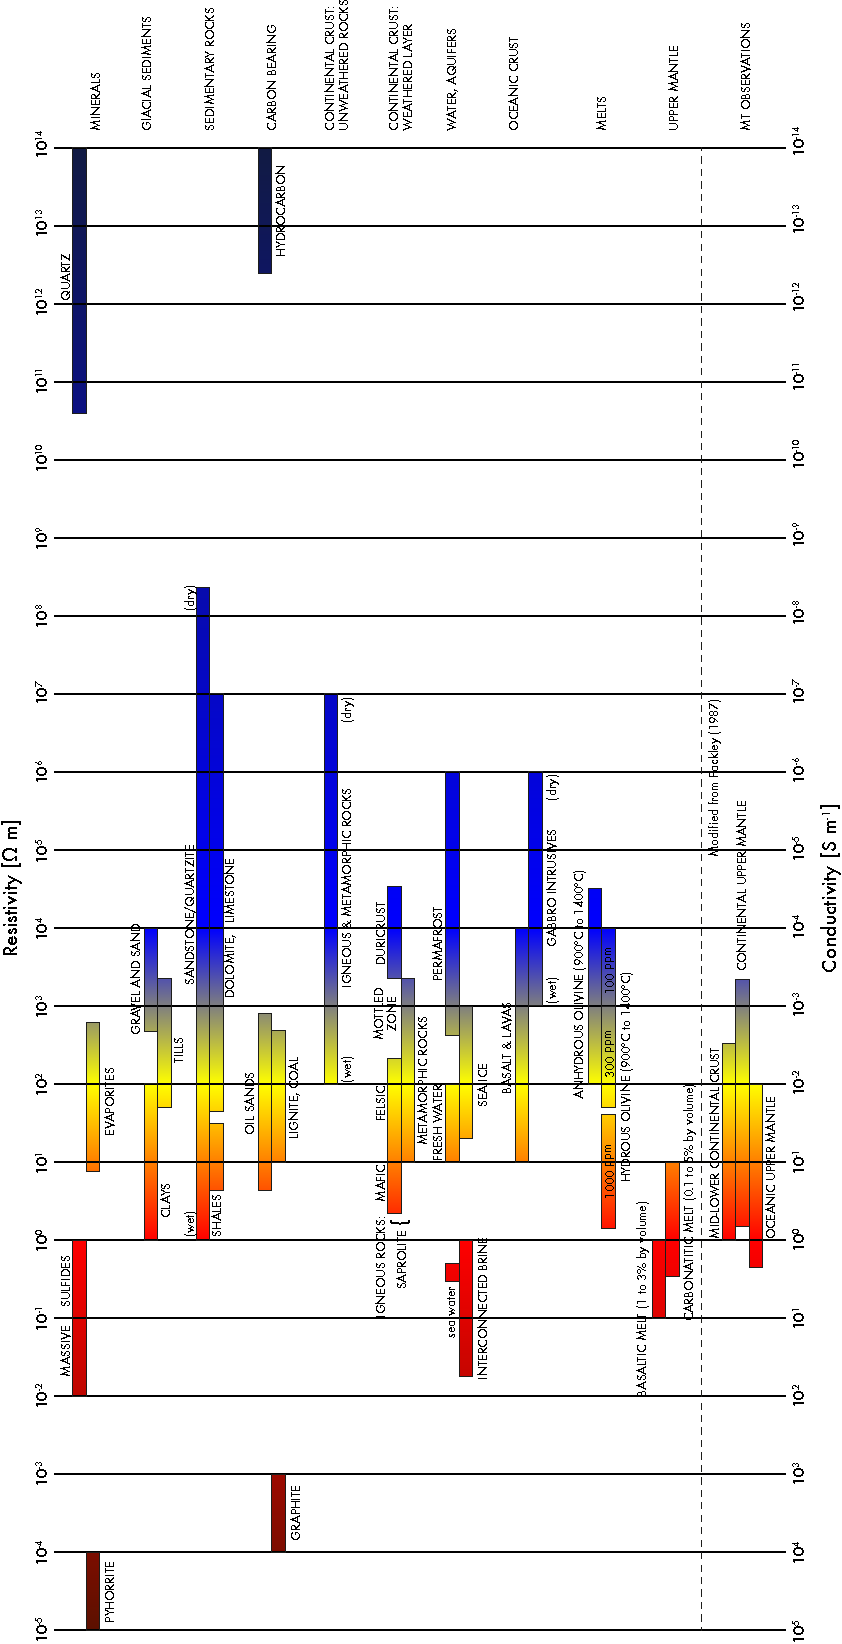
\includegraphics[height=0.95\textheight]{electromagnetics/figures/rock_resistivity.pdf}
    \caption{Resistivity of Earth materials.  Modified from \citet{Palacky1988,
    Telford_etal1990}.}
    \label{fig:rockrho}
\end{figure}

You may notice that the ranges of MT observations do not reach resistivity
values as high as those for most resistive materials or as low as most for
conductive materials.  There are few reasons for this discrepancy, (1) rocks
represent mixtures of both resistive and conductive components---conductive
minerals tend to be found in low concentrations and therefore often not well
interconnected---(2) some EM methods such as MT are insensitive to resistance
and hence never fully appreciate the high resistivities obtainable, and (3)
since many EM methods are diffusive, we model the effective conductivity over
very large volumes meaning extreme values are often smoothed.
\FloatBarrier

\subsection{Mixing Laws}
Mixing laws for conductivity are quite a bit more complex than they are for
other physical properties we have discussed.  The conductive component of
electrical conductivity can dominate conductivity at very low volume fractions,
sometimes at levels barely detectable except by chemical analysis.  There are
several mixing relations that are or have been used to estimate effective
electrical conductivity of mixtures.  We will focus on a small subset.

\subsubsection{Archie's Law}
Archie's law is technically a mixing relationship and widely used, but it has
very little sound physical basis and is instead an empirical relationship that
happens to capture some of the complexities related to the bulk resistivities of
mixtures.  Archie's law is given by
\begin{equation}
    \rho_{\mathrm{eff}} = \rho_f \phi^{-m},
\end{equation}
where $m$ is a constant, $\phi$ is the porosity, and $\rho_f$ is the
resistivity of the fluid filling the void.  For spherical particles, $m$ is
approximately 1.2; for sands, typically between 1.4 and 1.6; and for clays,
approximately 1.85, igneous rocks can have values closer to 2.6.  While Archie's
law can be a very useful relationship, it is empirical without a strong physical
basis.

Often within the petrophysical realm, the porosity term $\phi^{-m}$ is referred
to as the formation factor and used to help identify clay versus sand or other
content in borehole resistivity logs.

\subsubsection{Hashin-Shtrikman}
The Hashin-Shtrikman bounds are commonly quoted as a mixing relation for
electrical conductivity; however, the bounds often over- or under-predict the
conductivity, but that is what they are designed to do.  The bounds are
\begin{equation}
    \sigma_{\mathrm{HS}}^- = \mathcal{S}(\sigma_{\mathrm{min}}) \leq \sigma \leq
    \mathcal{S}(\sigma_{\mathrm{max}}) = \sigma_{\mathrm{HS}}^+,
\end{equation}
where $\mathcal{S}$ is defined as
\begin{equation}
    \mathcal{S}(x) =
    \Biggl( \sum_{i=1}^N \frac{\phi_i}{\sigma_i + 2x} \Biggr)^{-1} - 2x ,
\end{equation}
and $\phi_i$ is the volume fraction of the $i$-th component.

\begin{figure}[hbt]
    \centering
    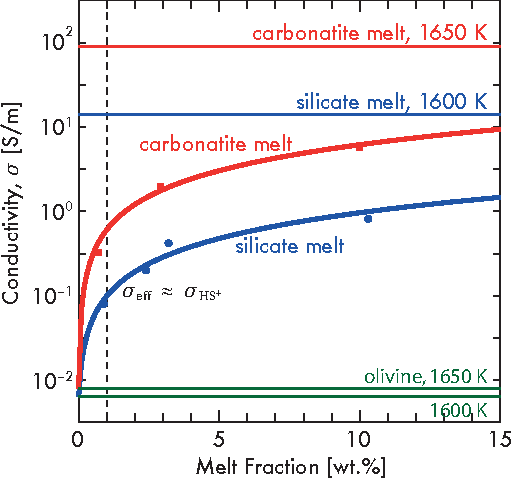
\includegraphics[]{electromagnetics/figures/melt_mixing.pdf}
    \caption{Electrical conductivity of basalt and carbonatite partial melts in
    an olivine matrix.  The results are predicted by the Hashin-Shtrikman upper
    bound.  Data from \citet{Yoshino_etal2010}.}
    \label{fig:sigmelt}
\end{figure}

\subsection{Solid Phase Conduction}
Electrical conduction occurs as charges are moved.  Generally, charges move in
response to a an applied electric or a changing magnetic field.  In solids,
moving charges requires energy, but in order for the charges to move an
activation energy (or minimum amount of energy) must be applied before the
charge will move.  The larger the activation energy, the lower the conductivity
(high resistivity).  Most charges in solid phase conduction result from the
movement of charge defects through a crystal.  Figure~\ref{fig:solidcond}
illustrates several important defects in the crystal olivine.
\begin{figure}[hbt]
    \centering
    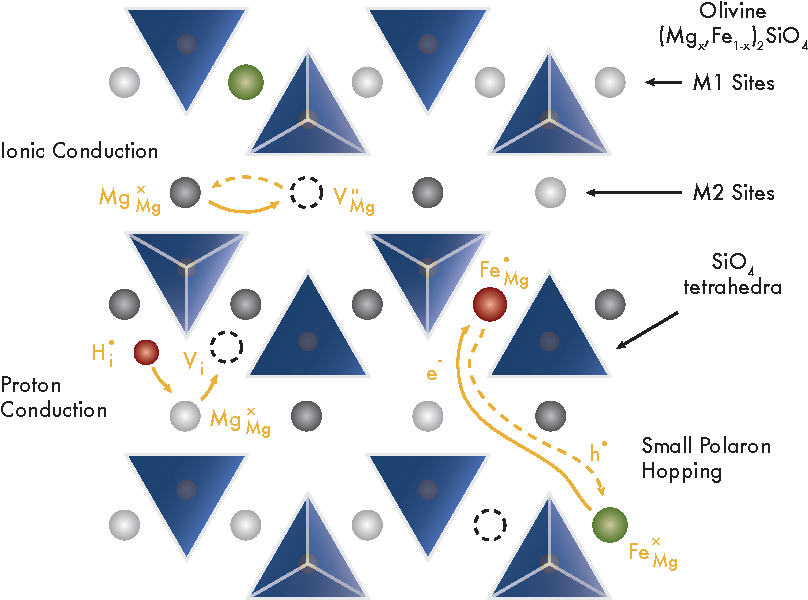
\includegraphics[]{electromagnetics/figures/conductivity_mechanism.pdf}
    \caption{Conduction mechanisms in olivine.  Conduction occurs by moving
    crystal defects through a crystal.}
    \label{fig:solidcond}
\end{figure}

The concentration of defects, $n_i$ with a crystal are temperature dependent,
\begin{equation}
    n = N \exp \left( - \frac{\Delta H_n}{k_B T} \right),
\end{equation}
where $N$ is the maximum number of defects, $\Delta H_n$ is the activation
enthalpy, $k_B$ is Boltzmann's constant, and $T$ is temperature in Kelvin.  We
describe the ability for charges to move by a parameter called mobility,
$\mu$, defined by
\begin{equation}
    \mu = m \exp \left( - \frac{\Delta H_\mu}{k_B T} \right) .
\end{equation}
where $m$ is the maximum mobility and $\Delta H_\mu$ is the activation
enthalpy.  Both the mobility and concentration can be used to determine the
electrical conductivity by
\begin{equation}
    \sigma_i = \sum_i n_i q_i \mu_i,
\end{equation}
where $i$ represents each charge defect.  For each conductivity mechanism, we
can write the electrical conductivity by a single relation,
\begin{equation}
    \sigma_i = \sigma_{0,i} \exp \left( - \frac{\Delta H_i}{k_B T} \right).
\end{equation}
The electrical conductivity due to any given defect can be expressed as a line
in $\log-\frac{1}{T}$ space,
\begin{equation}
    \log \sigma_i = \log \sigma_{0,i} - \frac{\Delta H_i}{k_B T} .
\end{equation}
This transform is convenient for plotting data as it makes it easy to observe
changes in dominant conduction mechanisms with increasing temperature
(Figure~\ref{fig:arrhenius}).  We call a $\log-\frac{1}{T}$ transform a
Arrhenius relation.
\begin{figure}[hbt]
    \centering
    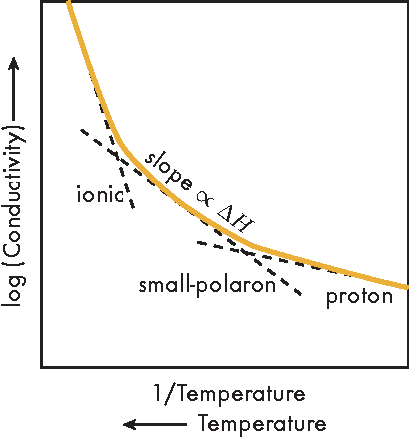
\includegraphics[]{electromagnetics/figures/arrhenius.pdf}
    \caption{Arrhenius diagram illustrating the addition the linear relationship
    between $\log$ conductivity and $1/T$.}
    \label{fig:arrhenius}
\end{figure}
The Arrhenius relationship for several mantle components is shown in
Figure~\ref{fig:sigmantle}.
\begin{figure}[hbt]
    \centering
    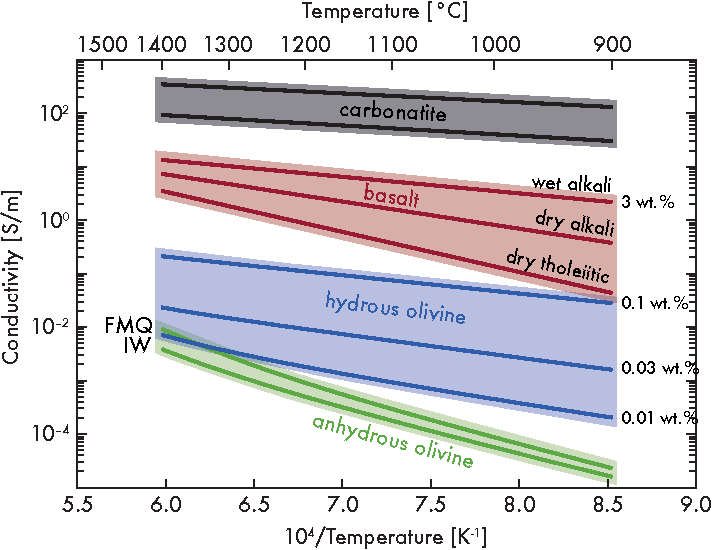
\includegraphics[]{electromagnetics/figures/mantle_conductivity.pdf}
    \caption{Arrhenius plot for conductivity of selected mantle materials.}
    \label{fig:sigmantle}
\end{figure}

\nocite{Jackson1999}
\nocite{Grant&West1965}
\nocite{Nabighian1991}

\FloatBarrier
\bibliographystyle{elsarticle-harv}
\bibliography{ref}
